\graphicspath{{content/chapters/3_methodology/methodology_figures}}

\chapter{Methodology}
\label{chp:methodology}

This section delves into the detailed approaches taken to achieve the project’s objectives, highlighting the reasoning behind each decision, and offering perspectives on the design and implementation of each objective.

\section{Data Integration and preprocessing}
\label{sec:3.1}

The preprocessing of raw data files is a crucial first step in any project. In this \acrshort{fyp}, we dealt with raw historical \acrshort{netcdf}~\cite{13} data spanning a total of four years, from January 2020 to December 2023 in hourly increments. The data was split into multiple folders and subfolders for each day, necessitating a robust method to merge and preprocess the data without interfering with its temporal and spatial dimensionality.

To address this, we developed a framework that allows us to specify the start and end dates for the required merging of the \acrshort{ssc} data. The framework then merges the individual files along the time dimension, creating a single comprehensive dataset that encompasses all relevant data across the specified interval. This merged dataset is not only more manageable but also streamlined for any subsequent processes.

A key feature of our framework is the preservation of the geographical boundaries and temporal aspects of the data. The dataset maintains the latitude and longitude ranges, ensuring the spatial integrity of the data is uncompromised. Similarly, checks were performed to ensure the time remained consistent, preserving the temporal integrity of the data.

Upon analysing the data, a substantial number of \acrshort{nan} values were discovered. These \acrshort{nan}s are likely due to the proximity of the data to the coast, where high-frequency radars  often struggle to capture all the data accurately. We decided not to address these \acrshort{nan} values at this stage, as each project objective requires specific handling of missing data, details of which will be explored in the respective sections.

This preprocessing framework was utilised in every section of the project, from the Lagrangian simulations, the AI models’ training and also the project’s evaluation. This underscores the critical role of preprocessing throughout the whole project. 

\section{Lagrangian Model Development}
\label{sec:3.2}

For this segment of the project, the OceanParcels toolkit~\cite{20} was utilised. The first step before proceeding with the simulation was to open the seven-day preprocessed \acrshort{ssc} dataset. Following this, the shapefile of Malta was loaded and used to create the land-sea mask. This mask, illustrated in Figure~\ref{fig_3.1}, was produced by rasterising~\cite{47} the coastline shapefile. This mask effectively differentiates land from sea, ensuring accurate particle tracking near coastal regions. The mask was then saved as a \acrshort{netcdf}~\cite{13} file and added within the grid boundaries to match with the boundaries of the dataset. These coastal boundaries are crucial for defining the simulation area and facilitating the implementation of land-sea interactions.

\begin{figure}[htbp]
    \centering
    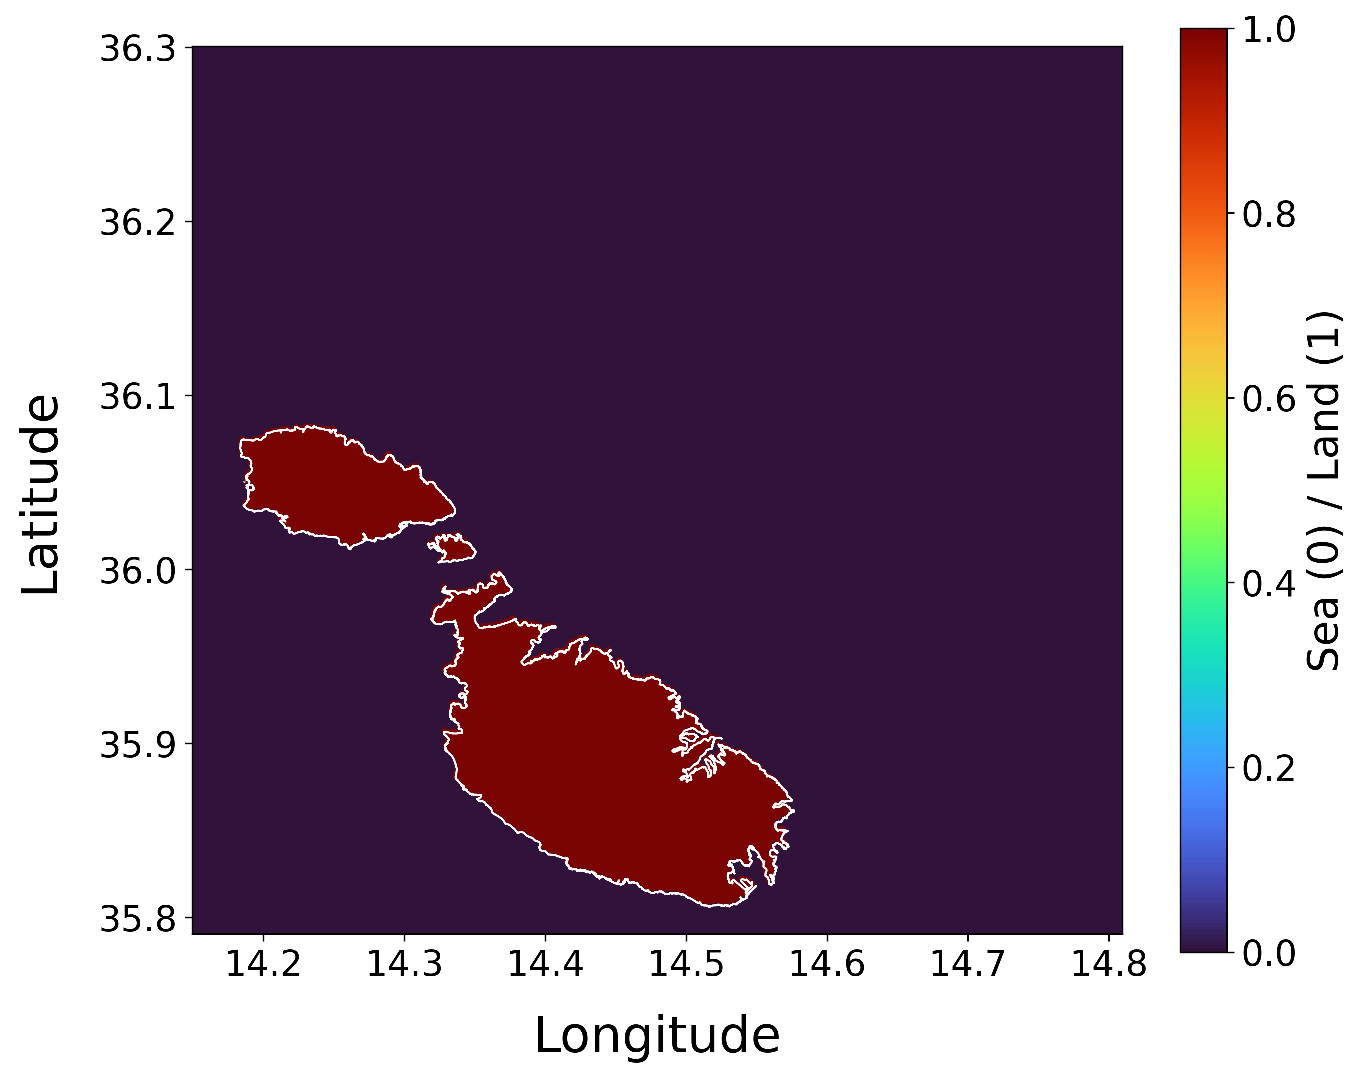
\includegraphics[width=0.5\textwidth,keepaspectratio]{land_sea_mask_malta.pdf}
    \caption[Land-sea mask of Malta.]{-- Land-sea mask of Malta.\label{fig_3.1}}
\end{figure}

Subsequently, a \textit{FieldSet} was created from the \acrshort{ssc} dataset. This serves as the simulation environment, defining the velocity fields that drive particle movement. Additionally, the land-sea mask was integrated into the \textit{FieldSet} as an additional field, providing the necessary data for reflecting or deleting particles upon reaching the coastline. As depicted in Figure~\ref{fig_3.2}, simulation particles were initialised near a specific geographic coordinate (36.0475°N, 14.5417°E), with random offsets to simulate a dispersed release. The particles represent the objects of interest, such as sea surface debris, whose movements are to be simulated. Initially, the strategy involved simulating numerous randomly placed particles across the entire area; however, to enhance realism, we placed 50 particles in close proximity. This configuration was selected to more accurately represent how clusters of debris navigate marine environments, with each particle representing a cluster of debris.

\begin{figure}[H]
    \centering
    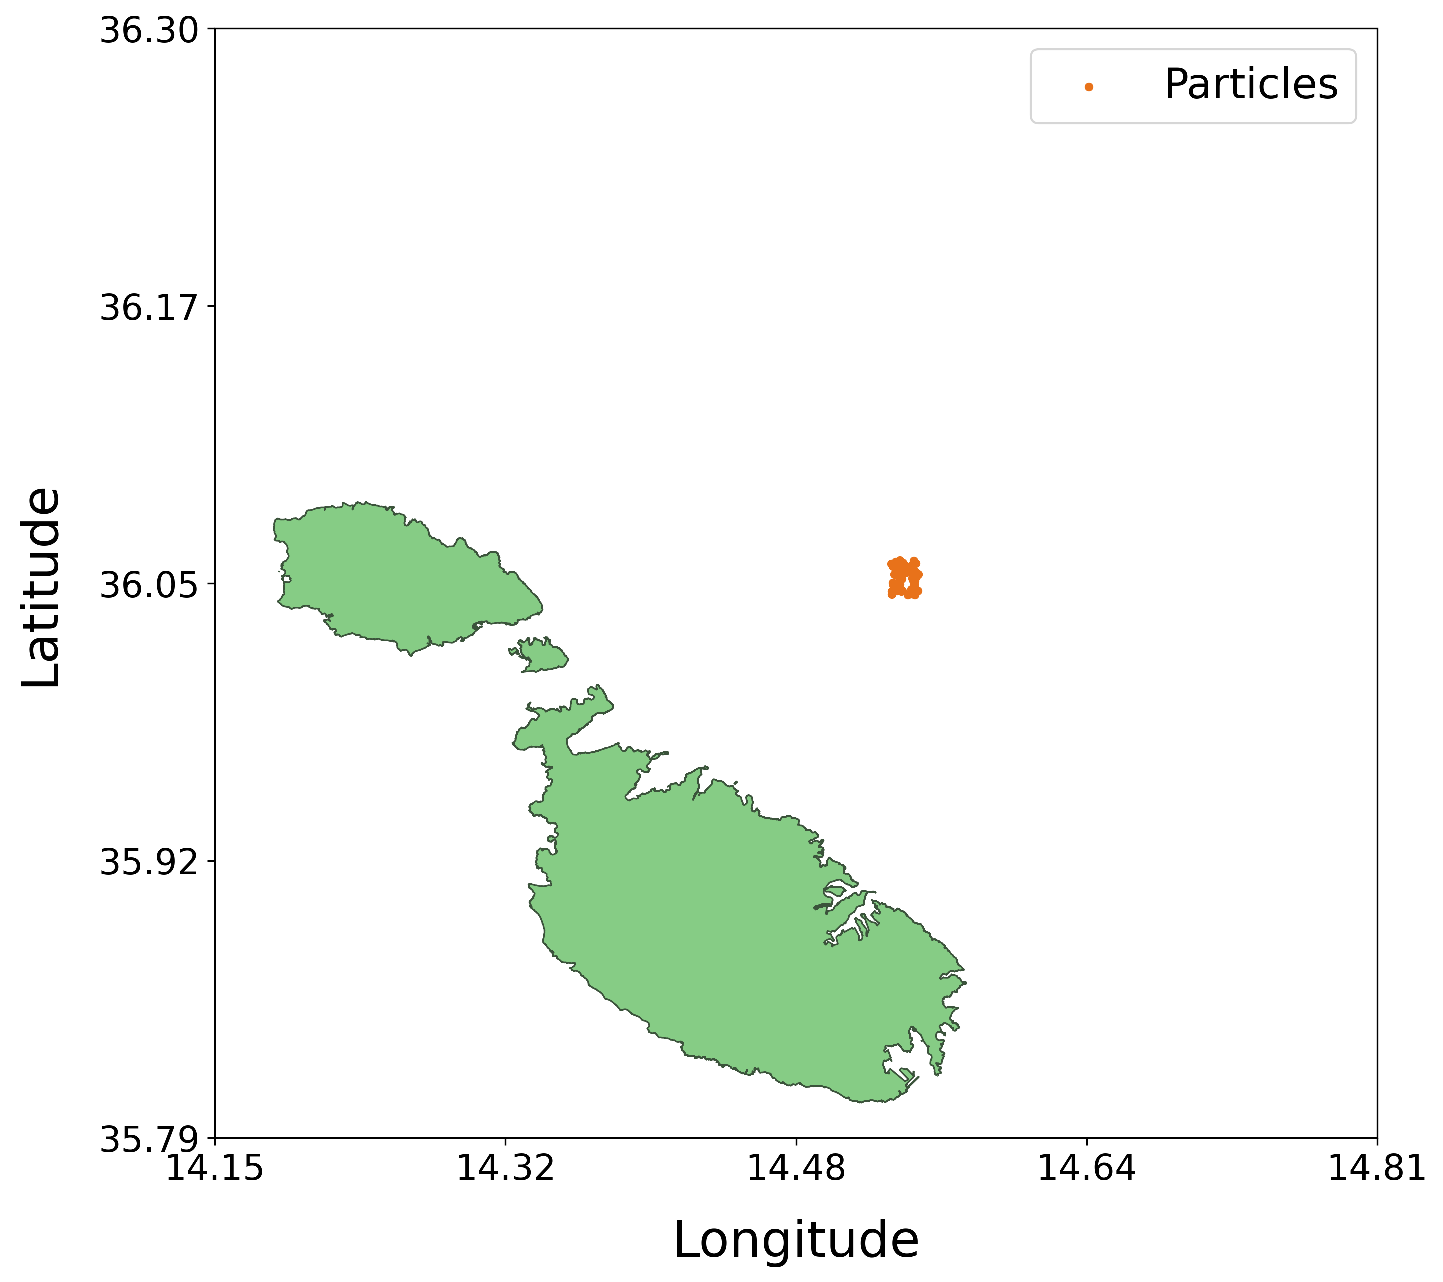
\includegraphics[width=0.5\textwidth,keepaspectratio]{initial_particle_locations.pdf}
    \caption[Initial particles locations.]{-- Initial particles locations.\label{fig_3.2}}
\end{figure}

The development and implementation of custom kernels was a critical component of the simulation. Custom kernels are scripts that introduce specific behaviours into the simulation, modelling realistic scenarios that particles may encounter. These behaviours include:

\begin{itemize}
    \item \textit{CheckOutOfBounds:} Deletes particles from the simulation if they move beyond the defined boundaries.
    \item \textit{CheckError:} Deletes particles encountering computational errors. This ensures the simulation proceeds without disrupted or incorrect particle data.
    \item \textit{UpdateElapsedTime:} Shows how long a particle has been in the system.
    \item \textit{UpdatePreviousPosition:} Captures the position of particles before they move.
    \item \textit{ReflectOnLand:} This function applies a reflection behaviour when particles encounter land, as defined by the land-sea mask. It also introduces a probabilistic component to interactions with land: there is a 15\% chance that particles will 'beach' and be removed from the simulation, while the remaining 85\% chance allows particles to be reflected back into the sea. This probabilistic distribution is informed by the geographic characteristics of Malta, where the predominance of rocky coastlines over sandy beaches increases the likelihood of debris being deflected back into the sea rather than beached.
\end{itemize}

The simulation was executed, and the resulting particle movements and dispersion patterns were visualised. These visualisations provide valuable insights into the trajectories of particles and their interactions with the environment. The time-step for the Lagrangian simulation is set at every 10 minutes, capturing the continuous dynamics of particle dispersion. The results are saved as a GIF file, offering a dynamic and easily interpretable visual representation of the simulated particle dispersion over time.

Some limitations emerged during this section of the project. Initially,  simulations revealed that particles were getting stuck at the border boundaries. This issue was traced back to the dataset, which lacked data at the borders, rendering the particles unresponsive to environmental variables in these areas. To address this, the boundary of the simulation area was slightly reduced by 0.1°. Originally, the intention was to run the simulation for three years. However, it became apparent that such a lengthy period was unnecessary and impractical for the project's goals. Therefore, this was adjusted to a more manageable seven-day simulation period. To achieve this, the preprocessing code from the previous section was utilised to merge the data from January 1 to January 7, 2023. Initially, the goal was to incorporate both wind and current data into the simulation, but we decided to only use the \acrshort{ssc} data. This decision was influenced by two main factors. Firstly, research like~\cite{48} indicates that sea surface debris is predominantly influenced by \acrshort{ssc} rather than wind. M. Erikson et al.~\cite{48} also suggest that while wind does play a role, it is less significant than \acrshort{ssc} in determining the spatial distribution of microplastics. Secondly, the complexity of integrating wind data and building custom behaviour kernels for wind interactions proved too challenging within the project's time frame. Despite this, it is recognised that including wind data could enhance the accuracy of the simulations in depicting real-life scenarios.

While addressing missing data, we encountered significant findings that shaped our approach. When we attempted to interpolate the data to fill in missing values, the visualisation results were noticeably different from those produced using the raw data which included \acrshort{nan}s. Despite experimenting with both linear and spline interpolation, the outcomes of the interpolated simulations remained consistent across different time frames, suggesting that the interpolation was homogenising the data excessively. This uniformity introduced by interpolation was misleading, as it failed to represent the true variability and dynamics of the ocean currents, obscuring the actual behaviour and movement patterns of particles in the sea. Consequently, we decided not to remove \acrshort{nan} values from the data used in the Lagrangian simulations. This decision was based on the understanding that removing or interpolating these values could lead to simulations that do not accurately reflect real-world conditions. By preserving the integrity of the original dataset, including its inherent gaps, the simulations are more likely to represent the actual conditions and variations that marine debris would encounter in the ocean. Examples of the final visualisations are presented in Figure~\ref{fig_3.9} and Figure~\ref{fig_4.8}.

The objective of initially implementing the Lagrangian model was to enhance our understanding and facilitate more informed decision-making for the subsequent sections. This exploratory phase was crucial in setting the stage for integrating more the AI models, ensuring that we had a solid foundation.

\section{AI Models Development}
\label{sec:3.3}

Predicting \acrshort{ssc} velocities is a crucial objective of this \acrshort{fyp}. Consequently, a comprehensive pipeline was established for this purpose. The initial phase involved selecting appropriate models, with \acrshort{lstm} and \acrshort{gru} architectures identified as optimal choices. This decision was informed by their demonstrated effectiveness in processing time-series data, rendering them particularly suitable for this task, as evidenced in studies like~\cite{42},~\cite{43}.

\subsection{Data Preprocessing and Geospatial Filtering}
\label{subsec:3.3.1}

This pipeline, outlined in Figure~\ref{fig_3.8}, forms the foundation of the project, playing an essential role in facilitating future predictions. The process begins with the preprocessing of the data. The initial plan was to train a model on a year's worth of data to forecast \acrshort{ssc} for the next month. However, the complexity and four-dimensional nature of the data led to sub-optimal predictions. Consequently, the strategy was revised to extend the dataset used for training, which now spans from February 25\textsuperscript{th}, 2020, to August 1\textsuperscript{st}, 2023. Given the substantial volume of data points and the need for geospatial filtering, a decision was made to concentrate on a smaller area of interest along the northern coast of Malta, as illustrated in Figure~\ref{fig_3.3}. The methodology involves predicting the \textit{'u'} and \textit{'v'} components individually for each longitude and latitude pair within this defined area. These individual predictions are subsequently merged into a unified file, which supports the execution of the subsequent Lagrangian simulation. This targeted approach, delineated by a specific polygon, ensures a more targeted and effective modelling process.

\begin{figure}[H]
    \centering
    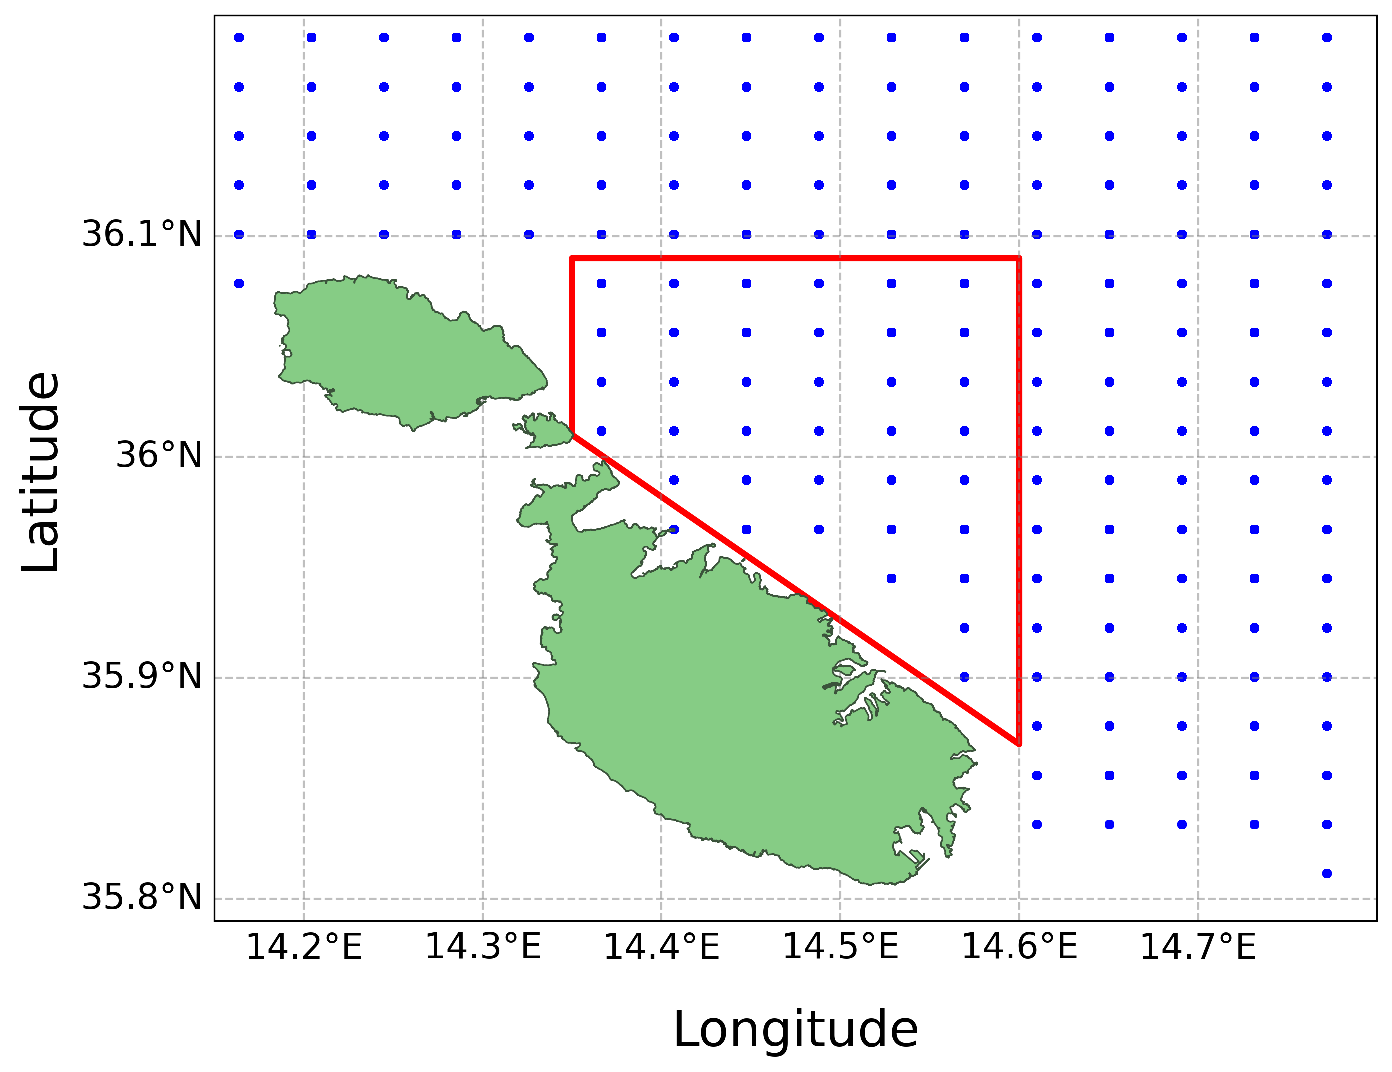
\includegraphics[width=0.5\textwidth,keepaspectratio]{all_data_points_and_selected_area_of_interest.pdf}
    \caption[All data points and selected area of interest.]{-- All data points and selected area of interest.\label{fig_3.3}}
\end{figure}

Next, the dataset was filtered to include only data points within the designated area of interest, as shown in Figure~\ref{fig_3.4}. This filtering resulted in a focused dataset consisting of 37 data points. Further preprocessing involved the removal of extraneous columns to streamline the dataset. Each coordinate pair was then processed into individual \acrshort{csv} files. These individual \acrshort{csv} files were systematically named and organised according to the corresponding latitude and longitude coordinate points. These files served as the basis for training the AI models for every individual data point.

\begin{figure}[H]
    \centering
    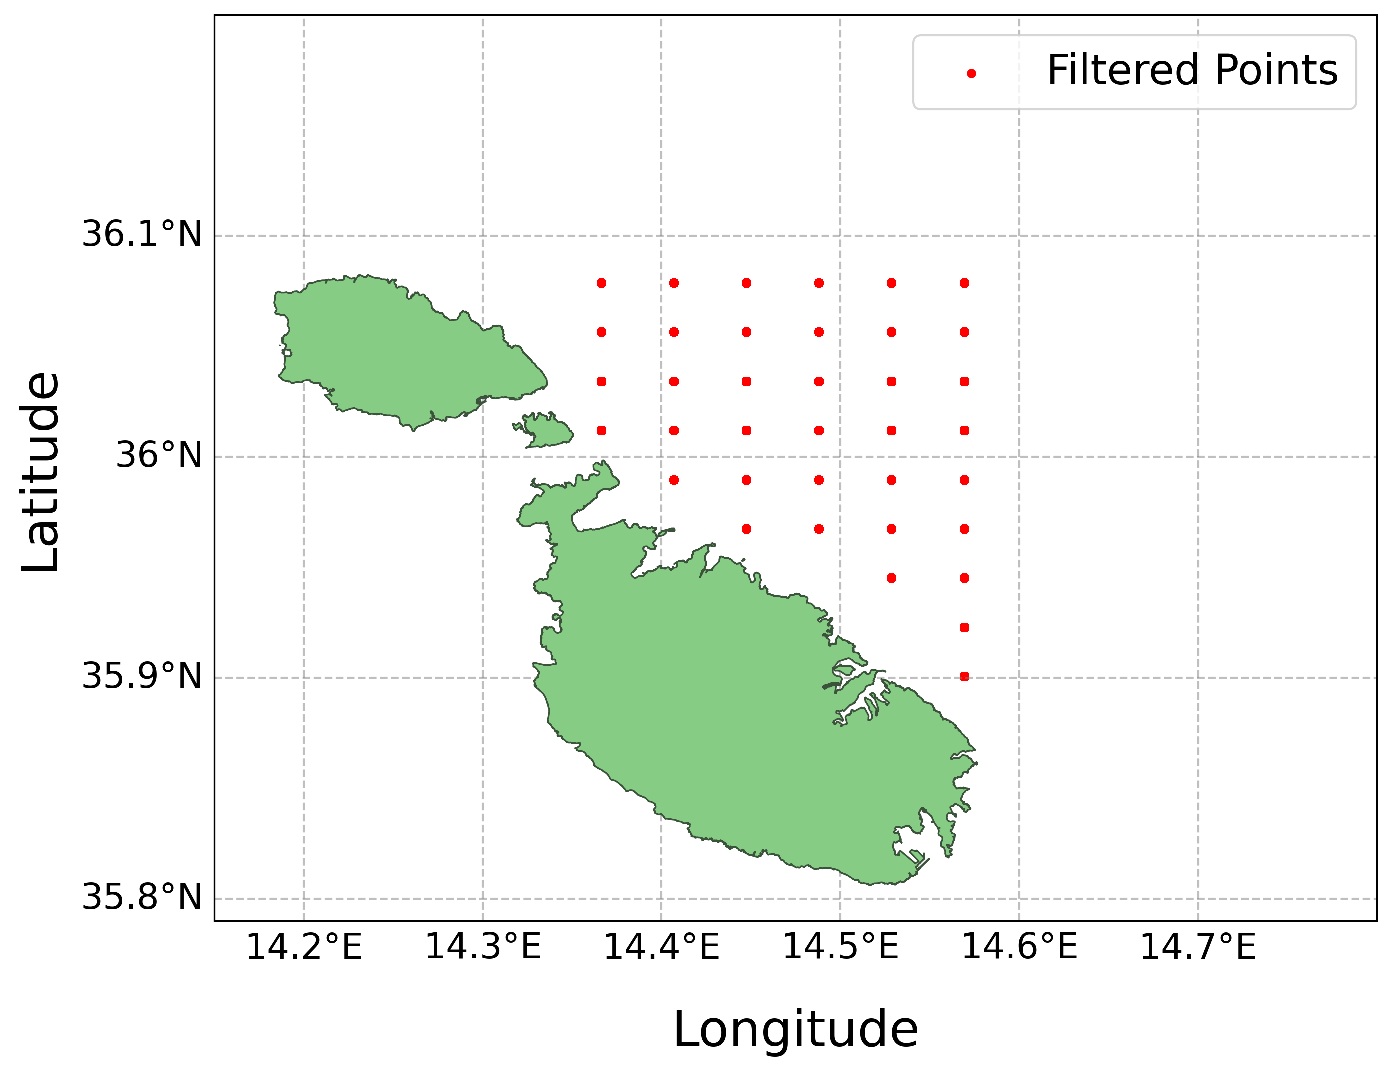
\includegraphics[width=0.5\textwidth,keepaspectratio]{filtered_points_within_area_of_interest.pdf}
    \caption[Filtered points within area of interest.]{-- Filtered points within area of interest.\label{fig_3.4}}
\end{figure}

In addressing missing data, we observed that areas closer to the coast exhibited fewer data points, as illustrated in the heat map (Figure~\ref{fig_3.5}). This scarcity of data near coastal regions is likely attributable to several factors: radar interference from nearby land or structures, obstruction of radar beams by coastal terrain or buildings, and refraction of radar waves at the coast, all of which could distort data collection. Efforts to solve this issue included experiments with data interpolation and filling missing values with the mean. However, these methods yielded worse results compared to those obtained by dropping the \acrshort{nan} values. Due to this, the most effective strategy proved to be the removal of \acrshort{nan} values, a decision informed by testing and also aligning with the methodologies applied in the Lagrangian model as discussed in section~\ref{sec:3.2}. 

\begin{figure}[htbp]
    \centering
    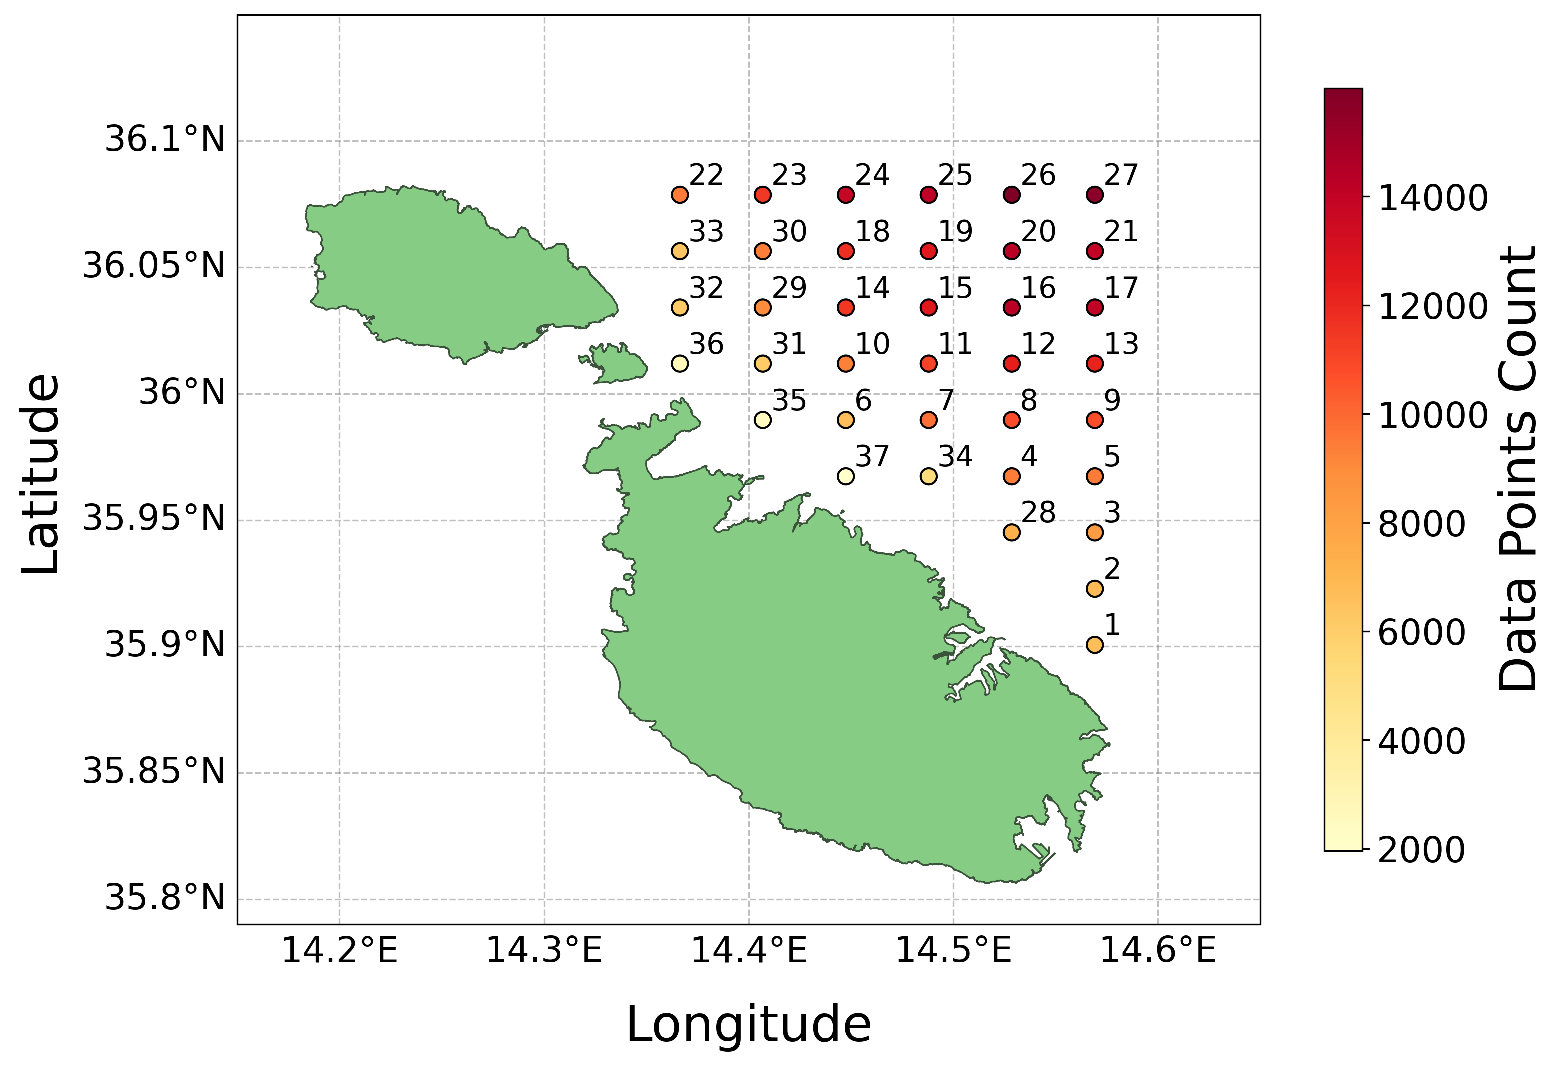
\includegraphics[width=0.5\textwidth,keepaspectratio]{amount_of_data_points_per_coordinate.pdf}
    \caption[Amount of data points per coordinate.]{-- Amount of data points per coordinate.\label{fig_3.5}}
\end{figure}

Prior to creating the pipeline, preliminary testing was conducted on a single model to determine the most effective features and targets. Experimentation involved the integration of both \textit{'u'} and \textit{'v'} as features, revealing marginally improved outcomes compared to using a single feature. Thus, it was determined that these components had a more significant impact, prompting a focus on using both features for predictions. Notably, the model yielded good results when predicting a single target. However, upon testing the model to predict both targets (\textit{'u'} and \textit{'v'}), the accuracy of predictions diminished noticeably. This observation led to the decision to develop separate models for each target variable to maximise the accuracy of the results. Therefore, we implemented a series of 37 models to predict the \textit{'u'} component, and this process was replicated for the \textit{'v'} component, ensuring precise and reliable predictions for each.

\subsection{The Main Loop}
\label{subsec:3.3.2}

Inspired by the approach in~\cite{44}, where the authors developed a model for every individual coordinate pair, we established a comprehensive pipeline that iterates through each pair of coordinates in the dataset and trains a dedicated model for each individual pair. This approach enables us to make predictions across the entire area of interest, which are later utilised in the Lagrangian simulations. The process begins by organising the \acrshort{csv} files according to their index. For each file, the \textit{'u'} and \textit{'v'} columns are extracted as input features. The dataset is then divided into training, validation, and testing segments in a 70-15-15 split respectively. Given the time series nature of the data, it was necessary to sequence the data appropriately, this was achieved using the \textit{TimeseriesGenerator} library. Extensive testing revealed that a window size of 72 hours, a batch size of 64, and a sampling rate of 1 yielded the best overall results. This means that the data is sequenced into continuous blocks of 72 hours of data as input and paired with the value immediately following these 72 hours as the target output. This crucial step allows the model to essentially predict the next hour based on the preceding 72 hours of data, a crucial step for accurate forecasting.

Various architectures and hyperparameters were also tested to find which gave the best results. For the comparison to be fair, we decided to use the same amount and type of layers and hyperparameters for both the \acrshort{lstm} and \acrshort{gru} architectures. Multiple architectural frameworks and hyperparameters were tested to ascertain the optimal configuration. To ensure a consistent basis for comparison, the same number, and types of layers, as well as hyperparameters, were employed across both \acrshort{lstm} and \acrshort{gru} models. The most effective architecture incorporated ten hidden layers, comprising four \acrshort{lstm}/\acrshort{gru} layers, three dropout layers, and two dense layers activated by \textit{ReLU}, followed by an additional dropout layer post each dense layer. The models were set up with a learning rate of 0.001, \textit{Adam} optimiser and \acrshort{mse} loss function. Importantly, the model was reinitialised in each iteration of the loop, ensuring that each dataset was trained on a fresh instance without any residual weights from previous iterations. This approach is crucial when dealing with multiple datasets to avoid any data leakage or influence from previously trained models (clean slate training). It also helps maintain the integrity of the learning process for each distinct dataset. Early stopping with a patience of eight epochs was implemented to halt training and prevent overfitting. Model checkpoints were utilised to save the best-performing epoch automatically. After each training epoch, plots comparing training versus validation loss were generated to monitor the performance of each model. To ensure that each model was trained adequately, predictions were made on the test set and subsequently visualised through a graph comparing actual versus predicted values, as illustrated in Figure~\ref{fig_3.6}. Finally, adopting a similar evaluation approach to~\cite{23}, \acrshort{mae}, \acrshort{mse} and \acrshort{rmse} error metrics were computed and displayed to evaluate the model's performance on the test set.

\begin{figure}[htbp]
    \centering
    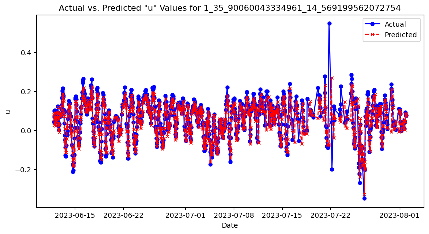
\includegraphics[width=0.7\textwidth,keepaspectratio]{actual_vs_predicted_values_on_test_set.pdf}
    \caption[Actual vs predicted values on test set.]{-- Actual vs predicted values on test set.\label{fig_3.6}}
\end{figure}

\subsection{Making Real World Predictions}
\label{subsec:3.3.3}

In the final phase of the \acrshort{ai} model pipeline, we undertook a simulation mirroring a real-world scenario by feeding data spanning 72 hours to predict the subsequent 24 hours. We decided to use data from August 1\textsuperscript{st} to August 3\textsuperscript{rd}, 2023, as input, aiming to predict conditions for August 4\textsuperscript{th}, 2023. This setup allowed us to compare the predictions with actual historical data from our dataset. The process began with a loop to systematically extract \acrshort{ssc} data across three days for all 37 individual coordinate pairs. Subsequently, actual data for the following 24-hour period on August 4\textsuperscript{th} were extracted for comparative purposes, and both sets were saved as \acrshort{csv} files. Given the requirement for 72 consecutive hours of data to be able to make predictions and 24 hours for comparison, spline interpolation was employed to address any present \acrshort{nan} values, ensuring the dataset's completeness. Using the rolling forecasting method as illustrated in Figure~\ref{fig_3.7}, predictions were generated for the subsequent 24-hour period for the individual targets, either \textit{‘u’} or \textit{‘v’}. Given the use of rolling predictions and the inclusion of interpolated values, it is important to recognise that the accuracy of the predictions may be affected. This is because predictions based on interpolated data serve as inputs for subsequent forecasts, potentially diminishing their precision. This effect is particularly noticeable in longer-term predictions, where accuracy tends to decrease as the forecast horizon extends, highlighting a decline in prediction accuracy the further the prediction extends into the future.

\begin{figure}[htbp]
    \centering
    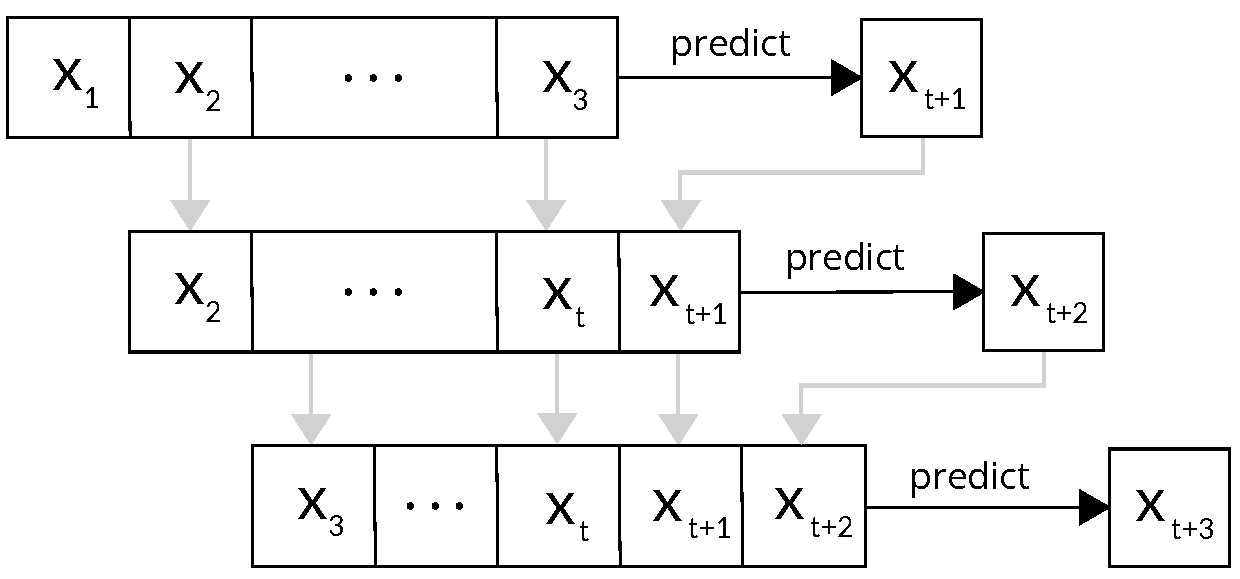
\includegraphics[width=0.5\textwidth,keepaspectratio]{the_process_of_rolling_forecast.pdf}
    \caption[The process of rolling forecast.]{-- The process of rolling forecast.\label{fig_3.7}}
\end{figure}

This pipeline is repeated for all 37 data points and then the predictions are converted into \acrshort{netcdf} format to be subsequently used for the Lagrangian model. Finally, the same error metrics are calculated and printed, to be used later for the evaluation. This pipeline was replicated four times, encompassing two \acrshort{lstm} models and two \acrshort{gru} models, one for each of the \textit{'u'} and \textit{'v'} components respectively.

\subsection{Pipeline Overview}
\label{subsec:3.3.4}

This subsection presents an overview of the \acrshort{ai} model pipeline (Figure~\ref{fig_3.8}). 

\begin{figure}[htbp]
    \centering
    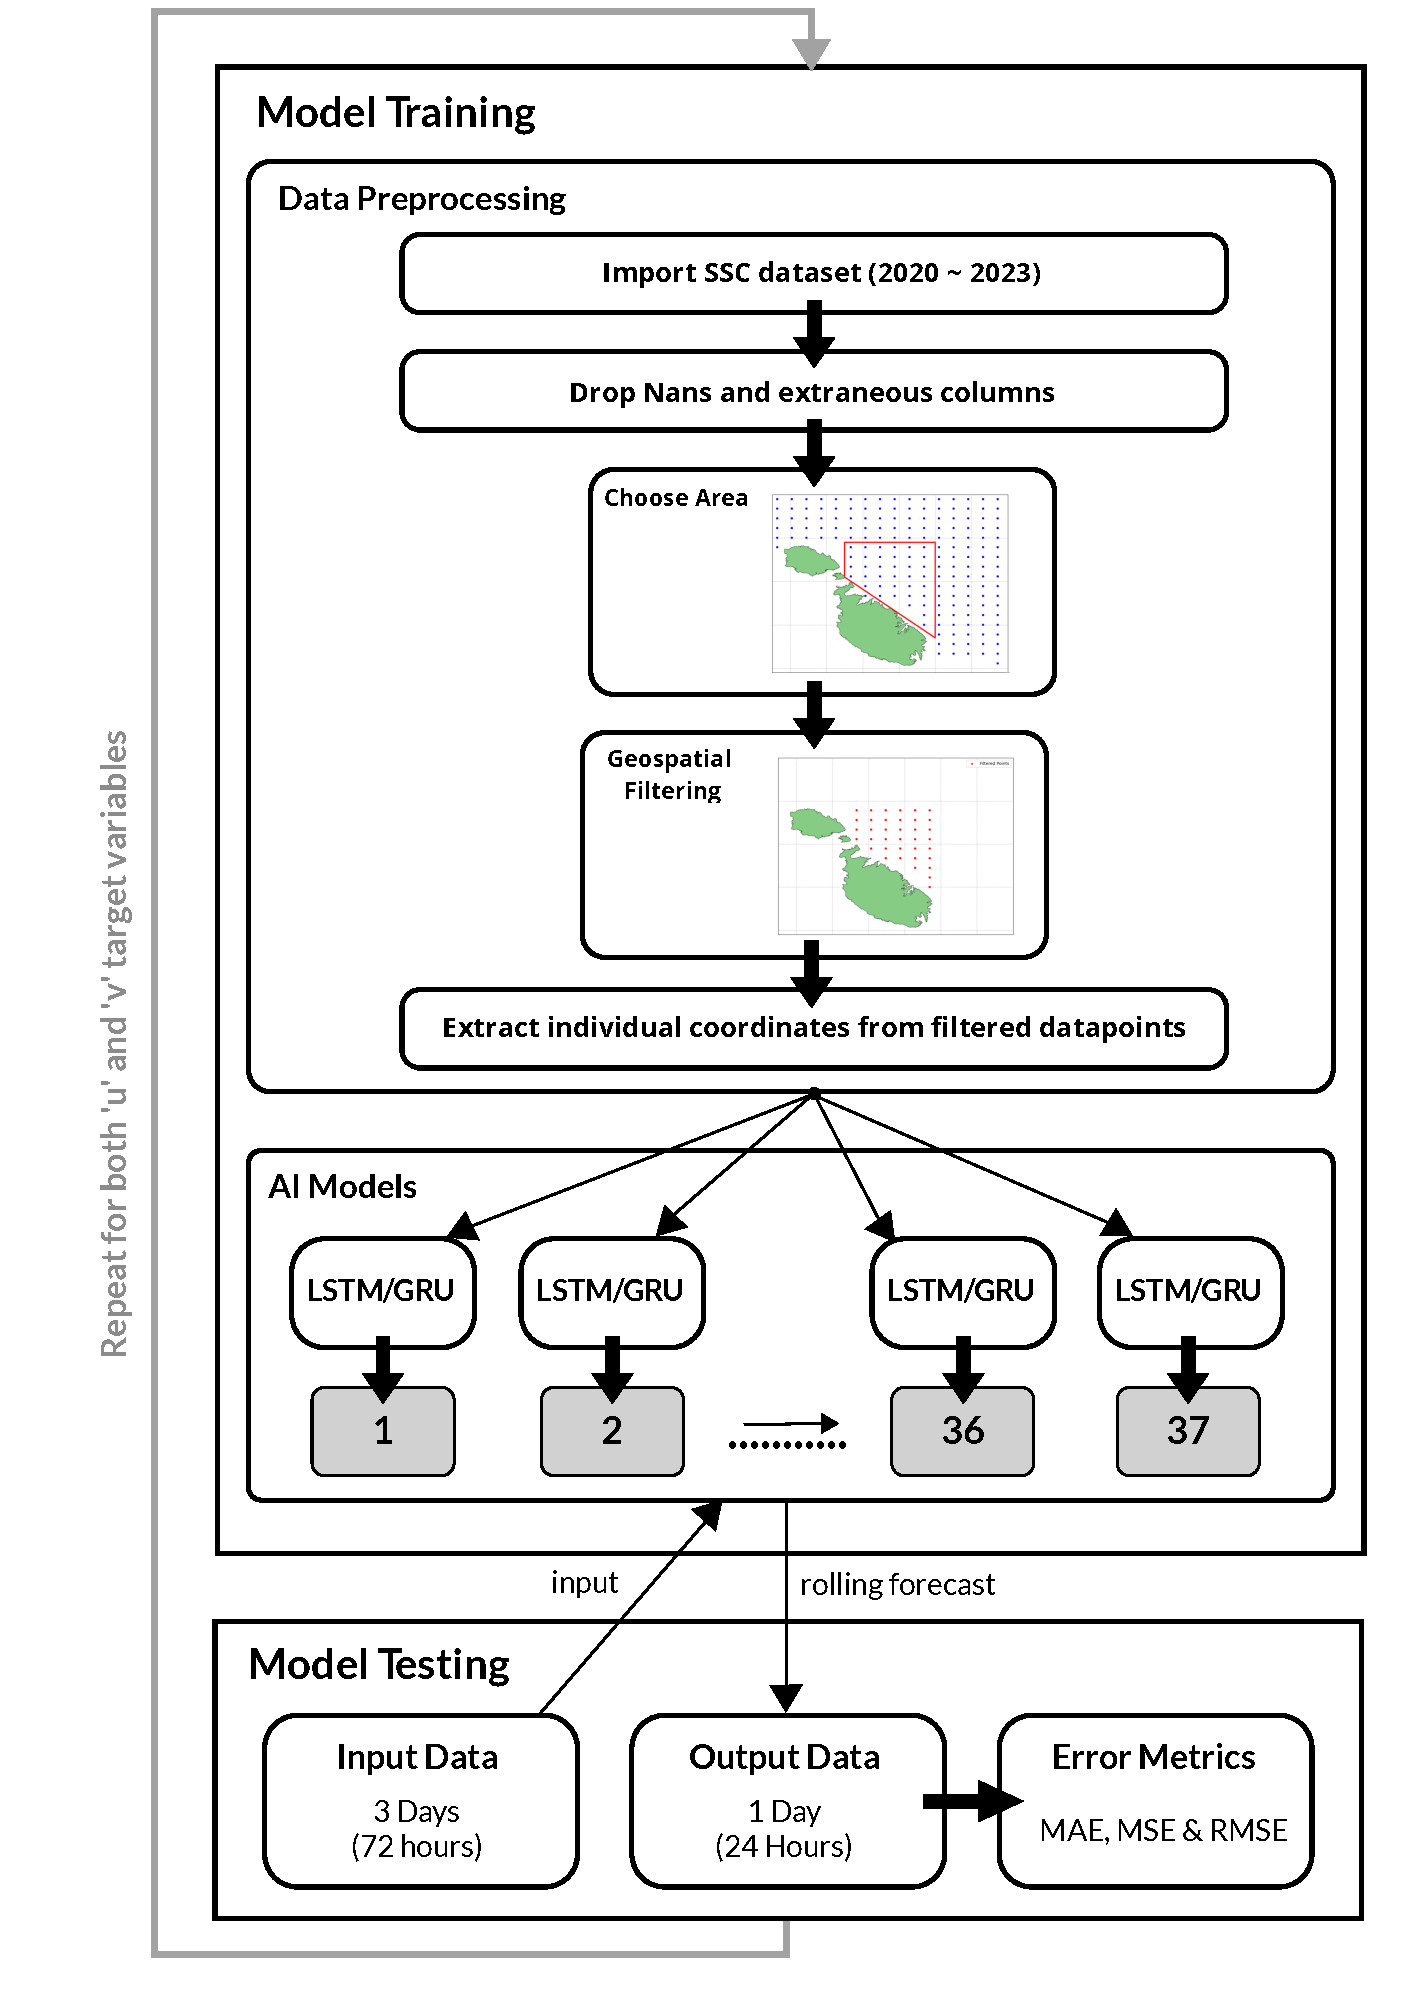
\includegraphics[width=0.2\textwidth,keepaspectratio]{overview_of_entire_AI_model_pipeline.pdf}
    \caption[Overview of entire AI model pipeline.]{-- Overview of entire \acrshort{ai} model pipeline.\label{fig_3.8}}
\end{figure}

\section{Integrating AI models with Lagrangian Model}
\label{sec:3.4}

The final stage of the pipeline is crucial. It involves the integration of the predictions generated by the AI models with the physics-based Lagrangian model to produce a 24-hour forecast simulation of sea surface debris dispersion.

This process was conducted separately for both the \acrshort{lstm} and \acrshort{gru} model predictions. The initial and most critical step involved the preprocessing and merging of the predicted \textit{'u'} and \textit{'v'} values. Multiple checks were implemented to ensure that the merging process was done correctly. The merged dataset was subsequently converted into \acrshort{netcdf} format. Following this, the procedures outlined in Section~\ref{sec:3.2} were implemented once again to set up the Lagrangian simulation. This involved the configuration of the land-sea mask, \textit{FieldSet}, number of particles, kernels, and timestep in a manner identical to the previous setup. The only difference lies in the particle initialisation phase. Given that the \acrshort{ai} model predictions are specific to the area of interest (as depicted in Figure~\ref{fig_3.4}), we decided to set the centroid of the polygon as the starting position. More specifically, the coordinates are at latitude of 35.9895° and a longitude of 14.4944°. This approach is advantageous as it allows for an unbiased observation of dispersion patterns. The reason being, since the centroid is equidistant from all edges of the polygon, it provides a neutral starting point that does not inherently favour any flow direction. In terms of the offset of the initial particles, the same random seed was employed for both \acrshort{lstm} and \acrshort{gru} simulations. This ensures a fair comparison as the initial locations of the particles are identical for both.

Finally, the Lagrangian simulations for both \acrshort{lstm} and \acrshort{gru} were executed and stored. The resulting particle movements and dispersion patterns were visualised and saved as \textit{GIFs}. These visualisations (Figure~\ref{fig_3.9}), allow us to observe the surface debris movement predictions. They also facilitate the evaluation of the results produced by the \acrshort{lstm} and \acrshort{gru} models respectively. 

\begin{figure}[htbp]
    \centering
    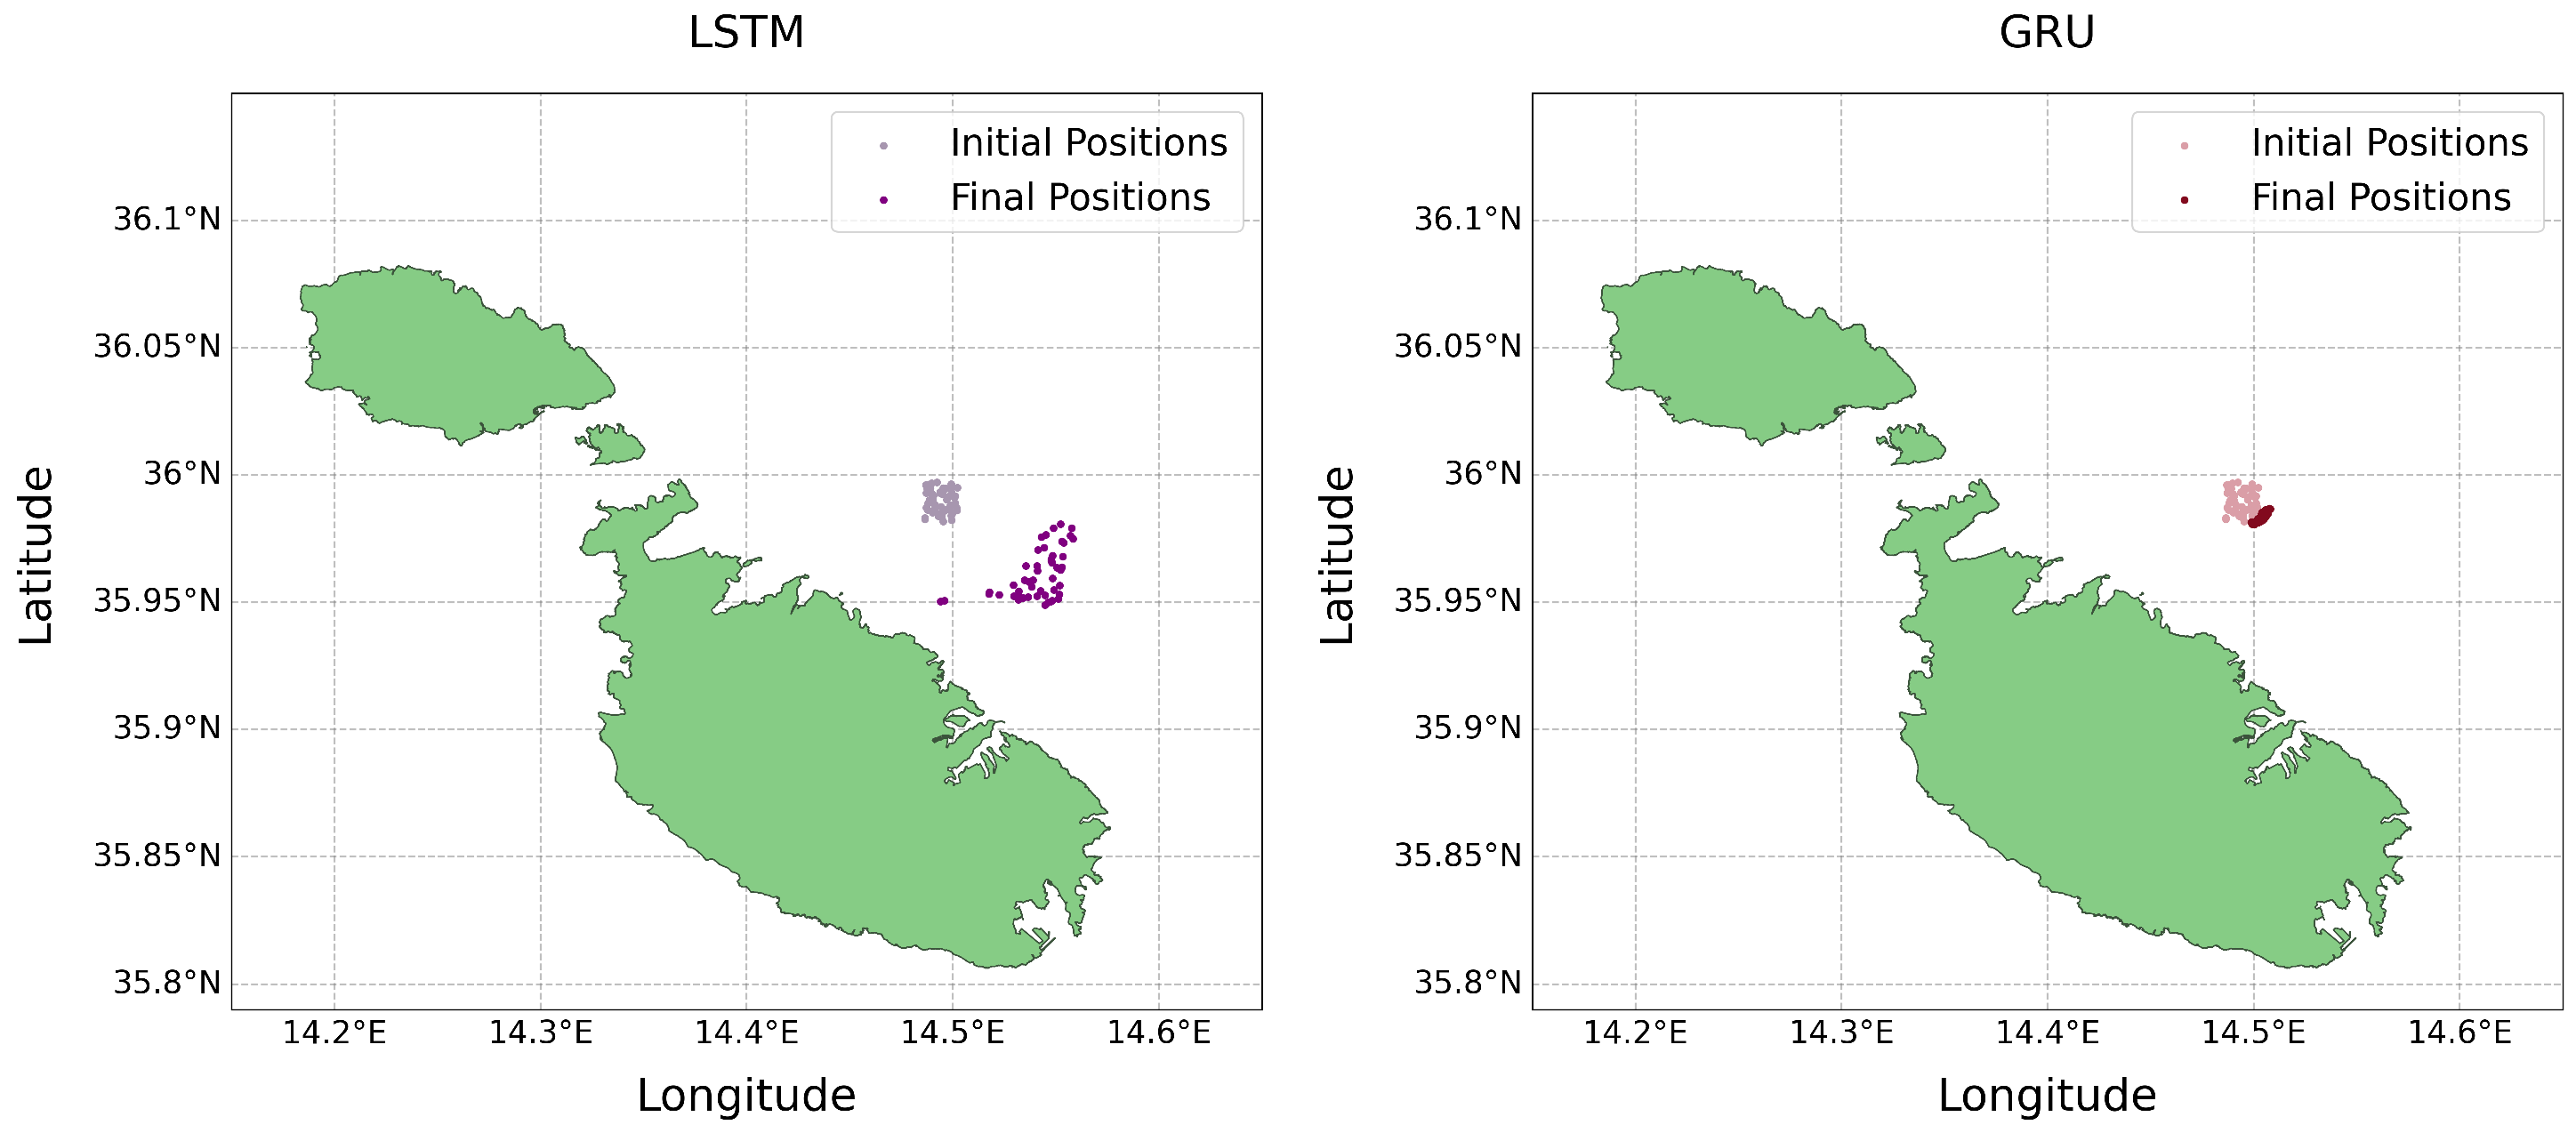
\includegraphics[width=0.8\textwidth,keepaspectratio]{LSMT_and_GRU_initial_vs_final_debris_movement_(August).pdf}
    \caption[LSTM and GRU initial vs final debris movement (August).]{-- \acrshort{lstm} and \acrshort{gru} initial vs final debris movement (August).\label{fig_3.9}}
\end{figure}

\section{Evaluation Strategy}
\label{sec:3.5}

The last phase of the \acrshort{fyp} focuses on a comparative evaluation between \acrshort{lstm} and \acrshort{gru} models' predictions. We required a way to test the performance of the models in a fair way to facilitate the comparison of the predicted results, allowing us to determine which model performed best.

Originally we also wanted to evaluate the Lagrangian framework by comparing dispersion patterns with drifter data, as undertaken in previous research~\cite{34,38}. However, due to the coastal proximity of our area of interest and the general practice of deploying drifters in open waters to avoid beaching, the drifter data was not available for our specific area. While it would have been the optimal approach to assess the Lagrangian simulations, we were unable to do so due to the unavailability of the necessary data. Instead, we decided to shift focus solely on the comparative analysis of \acrshort{lstm} and \acrshort{gru} model predictions. The accuracy of these predictions was evaluated using various error metrics to establish a comparative baseline. Furthermore, a spatial evaluation was incorporated to examine the similarity between the predicted dispersion patterns generated by each model.

To enhance the evaluation process, we opted to re-run the pipeline to predict \acrshort{ssc} for an alternate time period. Specifically, we inputted interpolated data spanning from November 1\textsuperscript{st} to November 3\textsuperscript{rd}, 2023, into the pipeline and utilising the trained models generated predictions for a 24-hour period for November 4\textsuperscript{th}, 2023. This allowed us to have two evaluation frame works for two separate dates, thereby facilitating a more comprehensive evaluation of the results. 

\subsection{Error Metrics Evaluation}
\label{subsec:3.5.1}

Adopting an approach similar to that described in~\cite{49}, we developed a concise pipeline to assess the predictive accuracy of the \acrshort{lstm} and \acrshort{gru} models. We utilised error metrics to compare the actual historical values versus the predicted values. specifically, we used the \acrshort{mae}, \acrshort{mse} and \acrshort{rmse}:

\[
\text{MAE} = \left(\frac{1}{N}\right) \sum \left|y_i - \hat{y}\right|
\]
\[
\text{MSE} = \left(\frac{1}{N}\right) \sum \left(y_i - \hat{y}\right)^2
\]
\[
\text{RMSE} = \sqrt{\text{MSE}} = \sqrt{\left(\frac{1}{N}\right) \sum \left(y_i - \hat{y}\right)^2}
\]

Where $N$ is the number of observations or data points, $y_i$ is the actual value for the $i^\text{th}$ observation, and $\hat{y}$ is the predicted value for the $i^\text{th}$ observation. Given that our analysis included 37 distinct models for both the \textit{'u'} and \textit{'v'} components, we computed the average mean and standard deviation for each metric to facilitate a more comprehensive evaluation of the \acrshort{lstm} versus \acrshort{gru} results across two timeframes: August 4\textsuperscript{th} and November 4\textsuperscript{th}. During our analysis, we identified certain outliers within the results. To address this, we also calculated the average using the \acrshort{iqr}, focusing on the differences between the 75\textsuperscript{th} and 25\textsuperscript{th} percentiles for each metric, thereby obtaining a more robust mean that excluded these outliers.

\subsection{Geospatial Evaluation}
\label{subsec:3.5.2}

In the second phase of our evaluation process, we introduced geospatial evaluation to enhance the comparative analysis of the \acrshort{lstm} and \acrshort{gru} models. This was motivated by the observation that each specific data point within our area of interest yielded varied results. Initially, we generated a heat map (Figure~\ref{fig_3.5}) to delineate which model corresponded to each location and to quantify the amount of data available for each model. Subsequently, to further our analysis for both the \acrshort{lstm} and \acrshort{gru} models, we visualised the \acrshort{mae} values for the \textit{'u'} and \textit{'v'} components using additional heat maps. The choice of \acrshort{mae} as a metric was deliberate, as it provides a straightforward and uniformly interpretable measure that treats all errors equivalently. These visualisations were instrumental in comparing the spatial accuracy of the models, highlighting areas where each model exhibited better or worse performance. These findings were then compared with the original heat map to discern patterns and discrepancies. This comparative analysis was executed for the predictions corresponding to both August 4\textsuperscript{th} and November 4\textsuperscript{th}, 2023, facilitating a thorough assessment of each model across different temporal contexts.

In the final stage of our evaluation, we quantified the performance of the \acrshort{lstm} and \acrshort{gru} models across different regions by calculating their centroid, spread, and skewness for their respective Lagrangian simulation outputs. The specific measures employed included:

\begin{itemize}
    \item \textbf{Mean, Median, and Standard Deviation of Centroids:} We computed the geographical centroids of the merged predictions from both the \acrshort{lstm} and \acrshort{gru} models to assess the proximity of the final debris movement predictions generated by the two models. The Euclidean distances from these centroids were then analysed, with the mean, median, and standard deviation calculated. Smaller values suggested a higher degree of concurrence between the models' predictions.
    \item \textbf{Spread of \acrshort{lstm} and \acrshort{gru}:} The spatial spread was determined by calculating the standard deviation of distances from each model's centroid. This measure of dispersion provided insights into the distribution of prediction points, where a lower standard deviation indicated a tighter clustering around the centroid, thus reflecting a more consistent model performance across the area.
    \item \textbf{Longitudinal and Latitudinal Skewness of \acrshort{lstm} and \acrshort{gru}:} To understand the directional tendencies of the models' predictions, we calculated the skewness for the distribution of the prediction points' longitude and latitude. A skewness close to zero indicated a symmetrical distribution of prediction errors, whereas a positive or negative skewness value pointed to a systematic bias in a particular direction.
\end{itemize}

By analysing these statistical measures, we aimed to determine not only which model had lower error values on average but also how those errors were distributed across the spatial domain. This approach offers insights into whether one model consistently outperformed the other across the entire study area, and also explores whether the models exhibited particular strengths or weaknesses in distinct regions. A comprehensive explanation and analysis of these evaluation results are presented in the subsequent chapter.

\section{Summary}
\label{sec:3.6}

In this chapter, we outlined the methodology implemented for this \acrshort{fyp}, detailing the comprehensive approaches undertaken for data integration, preprocessing, and model development. We began by establishing a framework for merging and preprocessing historical data, ensuring the preservation of its temporal and spatial integrity. This sets the stage for the Lagrangian model simulations to simulate sea surface debris movements. Subsequently, we delved into the development of AI models, specifically \acrshort{lstm} and \acrshort{gru} architectures for predicting \acrshort{ssc} velocities. This involved a detailed setup of data preprocessing, geospatial filtering, and a methodical training process for each coordinate pair within our area of interest. The chapter concluded with the integration of these \acrshort{ai} model predictions with the Lagrangian simulations to forecast sea surface debris dispersion, followed by an evaluation strategy employing error metrics and geospatial analysis to assess the models' predictive accuracy and spatial distribution tendencies.